\documentclass{bmvc2k}

%% Enter your paper number here for the review copy
% \bmvcreviewcopy{??}

% \usepackage[brazilian]{babel}
\usepackage[utf8]{inputenc}

\title{Manipulação de imagens baseada\\na cor de um pixel selecionado}

% Enter the paper's authors in order
% \addauthor{Name}{email/homepage}{INSTITUTION_CODE}
\addauthor{Gustavo Barros 18/0064487}{gustavoasb@gmail.com}{1}


% Enter the institutions
% \addinstitution{Name\\Address}
\addinstitution{
  Departamento de Ci\^encia da Comptuta\c{c}\~ao\\
  Universidade de Bras\'{\i}lia\\
  Campus Darcy Ribeiro, Asa Norte\\
  Bras\'{\i}lia-DF, CEP 70910-900, Brazil,  
}

\runninghead{Gustavo, Barros}{Computer Vision Assignment -- \today}

% Any macro definitions you would like to include
% These are not defined in the style file, because they don't begin
% with \bmva, so they might conflict with the user's own macros.
% The \bmvaOneDot macro adds a full stop unless there is one in the
% text already.
\def\eg{\emph{e.g}\bmvaOneDot}
\def\Eg{\emph{E.g}\bmvaOneDot}
\def\etal{\emph{et al}\bmvaOneDot}

%-------------------------------------------------------------------------
% Document starts here
\begin{document}

\maketitle
%-------------------------------------------------------------------------
\section{Resumo}
\label{sec:intro}

O projeto visa a criação de um software que nos possibilite
realizar certas tarefas envolvidas com o processamento de imagens. Através
do uso da biblioteca OpenCV \cite{OpenCV}, foram implementadas 4 modalidades de códigos
com diferentes pontos de funcionamento. A primeira retorna as coordenadas
de um local selecionado pelo usuário na imagem, as subsequentes servem para
marcar de vermelho pixels com cores semelhantes ao local selecionado, 
usando distância euclediana. Essa ação pode ser aplicada em respectativamente 
imagens, vídeos e dispositivos de captura.
%-------------------------------------------------------------------------
\section{Introdução}

Os objetivos deste projeto estão focados na introdução à manipulação de
imagens, com o auxílio de bibliotecas como OpenCV e NumPy \cite{scipy}. O processamento
de imagens é essencial para a visão computacional, logo é fundamental certo
conhecimento sobre o assunto. 

\subsection{Execução do software}
Inicialmente, é necessário rodar o programa corretamente, na pasta {\bf src} vinda
com o arquivo comprimido, está localizado o arquivo {\bf main.py}, que precisa ser executado
através da seguinte linha de comando no terminal (necessário Python instalado no computador):
\begin{quote}
    \tt{python main.py}
\end{quote}

\subsection{Acessando as funcionalidades}
Após a execução, as opções disponíveis serão mostradas em inglês no terminal, bastando
digitar um número referente a uma opção e dar enter para inicia-la. Para finalizar
basta selecionar um caractere ou número não disponível, fazendo assim o programa
parar automaticamente.

\pagebreak

A primeira opção se refere a localização de um click com o botão esquerdo do mouse 
em uma imagem. Ao clicar em algum ponto, o programa deverá retornar no terminal
dados sobre o local clicado, como a posição referente a Linha (Eixo Y) e Coluna (Eixo X),
além de determinar automaticamente se a imagem está em tons de cinza ou não, e com base nisso
retornar o valor de intensidade ou RGB. 

A segunda, terceira e quarta podem ser explicadas de forma conjunta, pois
possuem rotinas parecidas. Estas tem como funcionalidade a localização de
pixels de cor semelhante, calculando a distância euclediana de seus valores
RGB, ou, em casos de imagens em tons de cinza, a diferença absoluta nos valores
de intesidade. Após o usuário clicar na imagem, o programa detecta os valores
do pixel clicado e os usa para obtenção de outros pixels com valores semelhantes como
explicado previamente, estes outros então são marcados de vermelho, permitindo assim
a criação de áreas de coloração parecida. 
%-------------------------------------------------------------------------
\section{Requisitos}

Foram citados nos tópicos anteriores tarefas a serem estabelecidas, a partir de
agora vamos nos referir a elas como Requisitos, que vão de 1 a 4.

Para o Requisito 1, o programa retorna a posição do click com o botão esquerdo do mouse
em uma imagem, além de valores de cor ou intensidade. 

\begin{figure}[h]
    \centering
    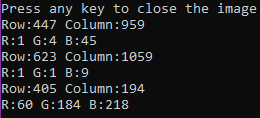
\includegraphics[scale=0.8]{Figs/r11.png}
    \caption{Exemplo de saída no terminal.}
\end{figure}

Uma parte importante desse requisito é que você precisa determinar se a imagem
está em tons de cinza ou não e a saída depende dessa informação. Para imagens coloridas
você dá os valores de RGB (Red,Green,Blue) e para o outro caso os valores de
intensidade. Para saber em qual modo está a imagem utilizamos a seguinte linha de código:

\begin{verbatim}
    if len(img.shape) > 2:
        grayscale = False
    else:
        grayscale = True
\end{verbatim}

Essa rotina vai ser repetida várias vezes durante os requisitos com o mesmo 
propósito. A função len retorna o tamanho do array e shape retorna os 
elementos da imagem {\em img}, como a altura, largura, e no caso de uma imagem colorida
um canal de cores. Por isso ao fazermos a comparação conseguimos determinar o modo da 
imagem, pois se ela estiver em tons de cinza terá apenas altura e largura como atributos, 
contabilizando 2.

\pagebreak

Depois de mostrar as imagens para o usuário é necessário detectar as ações do mouse, para isso
usa-se a função do OpenCV chamada setMouseCallback, setando o evento para ser o clique com o botão
esquerdo do mouse. Essa função já nos dá X e Y e usando eles chamamos outra função pixelInfo, que 
usando as coordenadas e a imagem original vê os valores de cor do pixel selecionado.

Para o Requisito 2 é necessário marcar de vermelho os pixels com cores semelhantes a do pixel clicado,
o sistema de obtenção de modo da imagem é praticamente identico ao da linha de código previamente mostrada,
porém quando uma imagem colorida tem o canal alpha nós descartamos ele. Além disso, se ela estiver em tons
de cinza é convertida para RGB a fim de poder-se pintar de vermelho.

A determinação que uma cor é semelhante a outra é feita através da distância euclediana \cite{Pbarrett}, que segue a
seguinte fórmula:
\begin{equation}
    d(q,p) = \sqrt{\sum_{i=1}^{n}(q_i - p_i)^2}
\end{equation}
Agora aplicando isso para o processamento da nossa imagem, temos que usar valores do RGB, deixando a fórmula
dessa forma:
\begin{equation}
    d = \sqrt{(r_1 - r_2)^2+(g_1 - g_2)^2+(b_1 - b_2)^2}
\end{equation}
Onde {\em r,g,b} com índice 1 são os canais Red, Blue e Green do pixel selecionado e os de índice 2 
do pixel que está sendo comparado.

No algoritmo estabelecido as operações são feitas através de operações entre 
matrizes, como podemos ver no fragmento de código abaixo (caso para imagens coloridas):
\begin{verbatim}
    mask = mask-pixel
    mask = np.square(mask)
    mask = np.sum(mask,axis=2)
    mask = np.sqrt(mask)
    mask = np.repeat(mask[...,None],3, axis=2)
    img = np.where(mask < 13, [0,0,255], img)
    return img
\end{verbatim}

Ao fazermos as operações matriciais nessa ordem estamos fazendo a distância euclediana
de forma indireta. Na quinta linha do fragmento podemos ver o uso do np.repeat, ele é usado pois
ao darmos np.sum na 3 linha estamos juntando os 3 canais de cores e formando apenas 1, e ao 
compararmos com a imagem original com 3 canais iremos ter problemas, logo usamos a função repeat
para repetir esse canal 3 vezes, operação que torna possivel usarmos as duas imagens
mask e img em conjunto para obtermos o resultado final. Onde {\em d} mostrado na equacão 2 for
menor que 13, pintamos de vermelho, operação feita na linha 6.

\pagebreak

O Requisito 3 usa mesmo efeito do Requisito 2 porém aplicado a vídeos, para faze-lo funcionar
em vídeos, é necessário criar um loop que lê cada frame do vídeo e faz o processo anterior para cada
um deles. O código dessa parte ficou da seguinte maneira:

\begin{verbatim}
    while(video.isOpened()):   
        ret, frame = video.read()
        mask = frame.copy()
        original = frame.copy()
        cv2.setMouseCallback('frame',mouseClick)
        if(pixel[0] != None):
            frame = paintPixels(frame,mask,pixel)
        cv2.imshow('frame', frame.astype(np.uint8))
        if cv2.waitKey(25) & 0xFF == ord('q'):
            break         
\end{verbatim}

Depois de lermos a imagem precisamos criar um loop que atualiza o vídeo, a função 
{\em read} faz isso a cada laço, ela retorna o frame, que é a imagem em que vamos aplicar
o efeito. Antes disso precisamos de duas cópias do frame, uma para retornarmos ao original,
e outra para fazermos cálculos encima. A função de {\em setMouseCallback} retorna os valores RGB
do local clicado para a variável pixel. Então quando pixel tiver um valor real será chamada a função
que pinta a imagem frame, função essa semelhante à usada no requisito 2.

O tempo que a imagem demora para ser atualizada é 25 milissegundos, tempo determinado pela função
{\em waitKey} na penúltima linha do fragmento. Na mesma linha temos a condição de break, determinada
para ser ativada pela tecla ``q'', dando opção assim pro usuário encerrar o vídeo.

O Requisito 4 é idêntico ao 3, porém aplicado a um dispositivo de captura, como uma webcam. A diferença
nessa caso será a entrada, que deixará de ser um vídeo. Na linha abaixo mostra-se como podemos usar um dispositivo
desses como entrada:
\begin{verbatim}
    cam = cv2.VideoCapture(0, cv2.CAP_DSHOW)
\end{verbatim}

Usando isso podemos seguir os mesmos passos do Requisito 3 e chegar ao resultado esperado.
%-------------------------------------------------------------------------

\section{Resultados}

A fim de demonstrar o funcionamento do programa e suas funcionalidades, 
alguns resultados serão demonstrados.

\subsection{Requisito 1}

O Requisito 1 é baseado em mostrar coordenadas de um local clicado e seus
atributos RGB ou de intensidade, para o teste vamos usar um exemplo.

Vamos selecinar dois pontos A e B. A sendo um local claro, e B um local mais escuro, assim
podemos analisar melhor a saída oferecida por cada um deles.

\pagebreak

\begin{figure}[h]
    \centering
    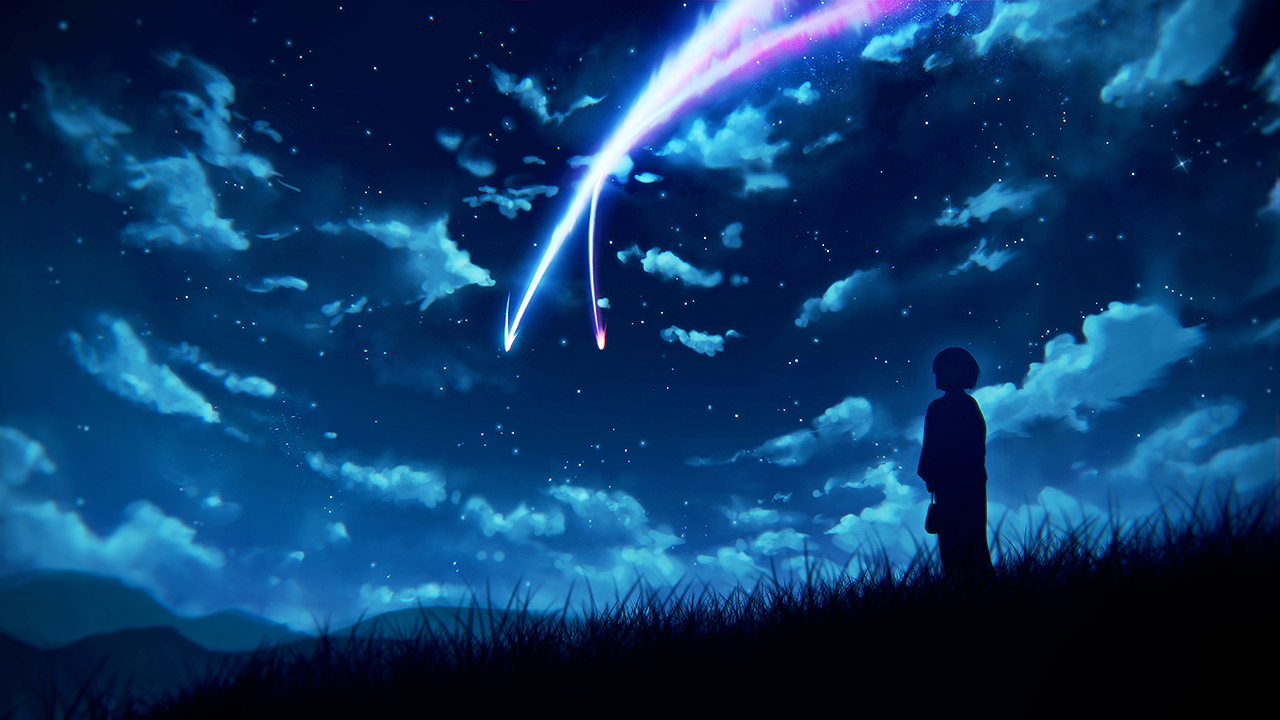
\includegraphics[scale=0.2]{../data/kiminonawa.jpg}
    \vspace*{-2mm}\caption{Imagem exemplo para teste do Requisito 1.}
    \vspace{0.1cm}
    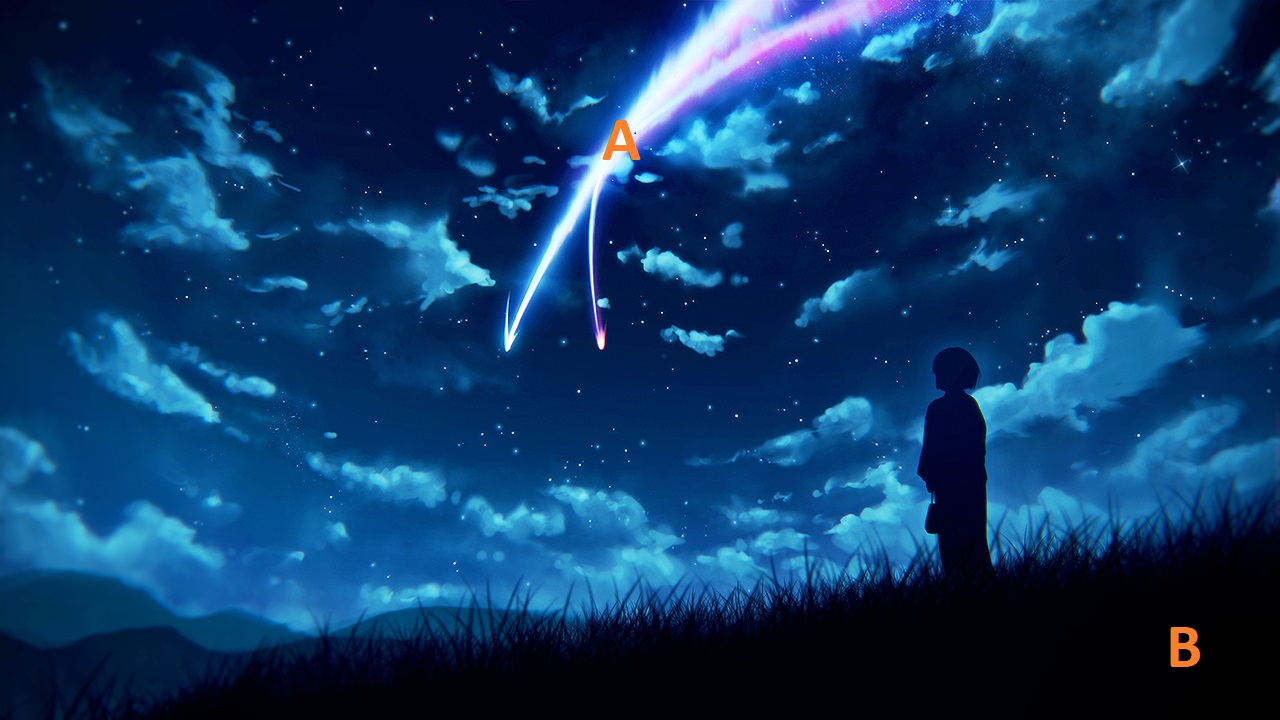
\includegraphics[scale=0.2]{Figs/r14.jpg}
    \vspace*{-2mm}\caption{Locais clicados para saída A e B.}
    \vspace{0.1cm}
    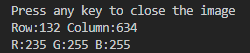
\includegraphics[scale=0.8]{Figs/r12.png}
    \vspace*{-2mm}\caption{Saída A.}
    \vspace{0.1cm}
    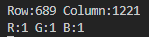
\includegraphics[scale=0.8]{Figs/r13.png}
    \vspace*{-2mm}\caption{Saída B.}
    \vspace{0.1cm}
\end{figure}

Olhando logo pelos valores R,G,B podemos perceber a diferença de intensidade
entre os locais clicados, o que bate com o esperado. Abaixo também um teste com uma imagem
em tons de cinza.

\begin{figure}[!h]
    \centering
    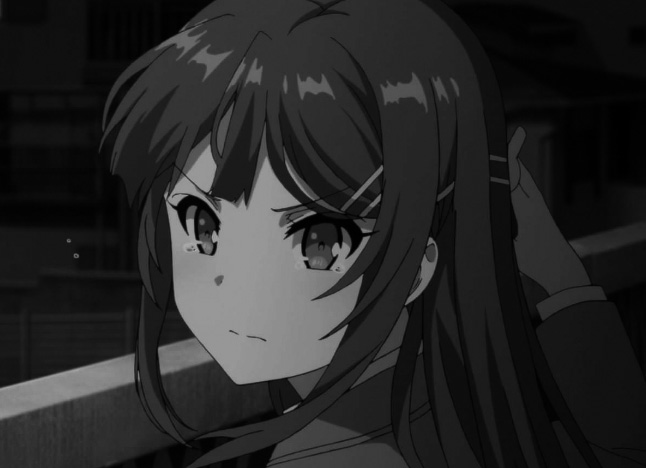
\includegraphics[width=0.300\textwidth]{Figs/maigray.jpg}
    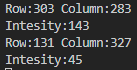
\includegraphics[width=0.300\textwidth]{Figs/r15.png}
    \vspace*{-2mm}\caption{Teste tons de cinza.}
\end{figure}

\subsection{Requisito 2, 3 e 4}

Como os Requisitos que sobraram tem funções parecidas mas diferentes locais alvo vamos
compara-los no mesmo tópico.

\begin{figure}[h]
    \centering
    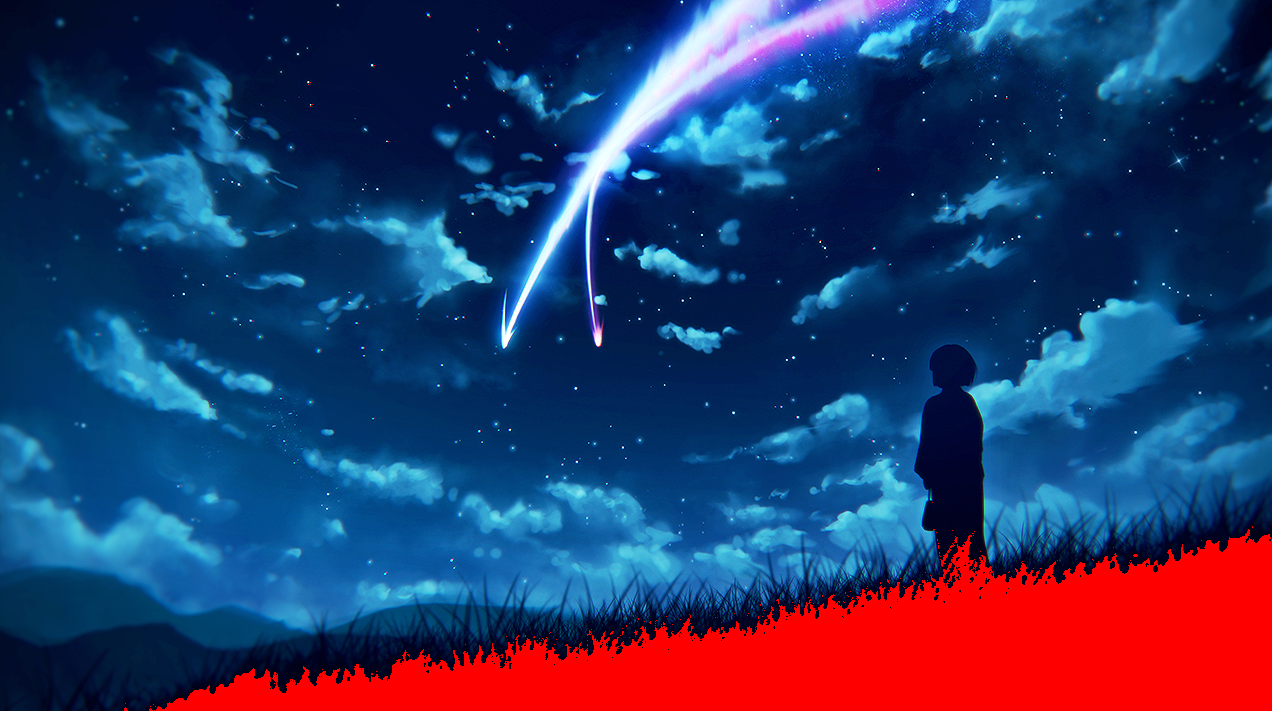
\includegraphics[scale=0.2]{Figs/r21.png}
    \vspace*{-2mm}\caption{Clique efetuado na grama.}
    \vspace{0.1cm}
    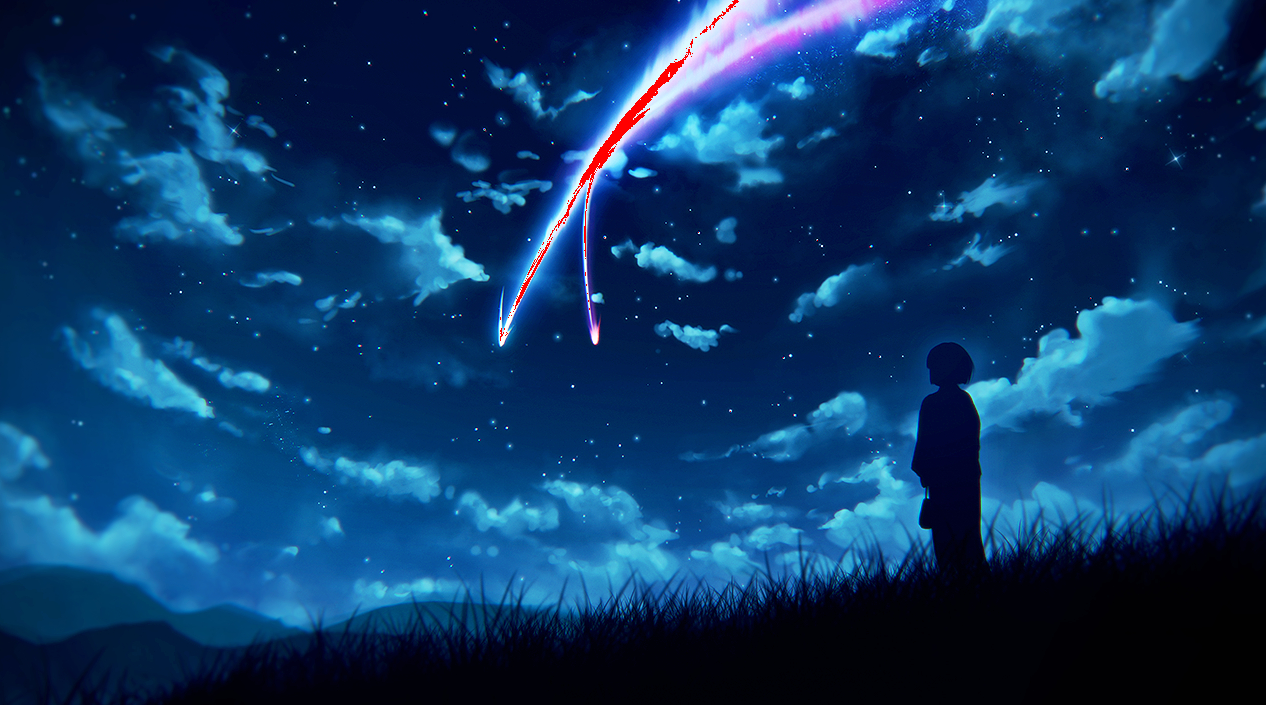
\includegraphics[scale=0.2]{Figs/r22.png}
    \vspace*{-2mm}\caption{Clique efetuado na luz do céu.}
    \vspace{0.1cm}
\end{figure}

Percebe-se que os locais de cores similar são marcados de vermelho, no caso acima 
esscolheu-se a luz e a grama por serem os locais com cores mais distintas do resto.

\begin{figure}[h]
    \centering
    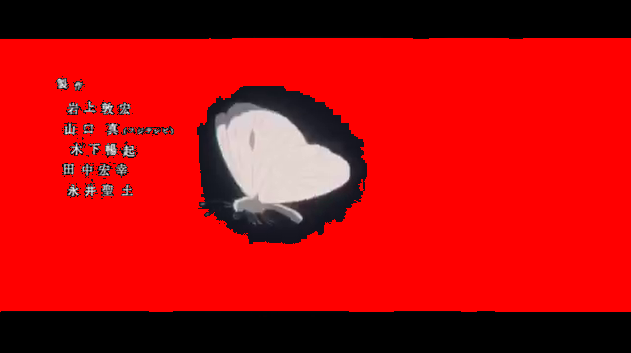
\includegraphics[scale=0.5]{Figs/r31.png}
    \vspace*{-2mm}\caption{Clique efetuado em vídeo teste.}
    \vspace{0.1cm}
\end{figure}

No caso acima foi testado o clique em um vídeo, funcionalidade do Requisito 3. No frame mostrado o fundo 
era predominantemente preto, o que destacou a borboleta, como pode ser visto 
pelo resultado final.

%\pagebreak

\begin{figure}[h]
    \centering
    
\includegraphics[scale=0.4]{Figs/r41.png}
    \vspace*{-2mm}\caption{Clique efetuado em dispositivo de captura.}
    \vspace{0.1cm}
\end{figure}

Como é visível na imagem acima, o local alvo foi uma webcam. Logo, pode-se ver que o monitor
foi quase completamente destacado, por ter uma cor preta semelhante.

\section{Discussão e Conclusões}

As aplicações desenvolvidas alcançaram o resultado esperado, não com máxima eficiência, porém com
suficiente para rodar o vídeo de forma fluída, assim como a webcam. 

A primeira parte do desenvolvimento não utilizava funcões do NumPy \cite{scipy} e sim laços, logo 
foi percebido que esse método era ineficiente, pois o tempo de processamento era muito
demorado. O vídeo utilizando esse método anterior tinha sua fluidez prejudicada e
ficava com uma baixa taxa de quadros por segundo.

Também foi percebido problemas com unidades de armazenamento, principalmente
pelo uso do uint8, logo foram resolvidos inúmeros conflitos fazendo casting
ou adaptando para o uso do tipo de variável anteriormente mencionada.

Percebe-se que o programa é eficaz quando há grande distinção de cores, podendo até 
destacar um objeto em um plano, como pode ser visto na {Figura 9}.

Concluimos então que o software desenvolvido atende ao que foi pedido, tendo a capacidade
de realizar os 4 requisitos estipulados. Houve também grande avanço no entendimento da 
biblioteca OpenCV \cite{OpenCV}, que auxílio na manipulação de imagens.

Pode-se dizer que a ordem em que o projeto foi desenvolvido colaborou para a aprendizagem, pois 
a ordem de cada tarefa fez com que a anterior fosse necessária para o cumprimento da 
próxima.

Os conceitos de RGB \cite{geraldbakker} \cite{blind}, tons de cinza, assim como a realização correta de operações matriciais, foram estremamente importantes
para o entendimento das atividades e sua realização. A distinção do modo de imagem
nos deixou claro como todas as informações de uma imagem ficam armazenadas, além de
demonstrar como o computador interpreta uma imagem e como ele guarda as informações dela. A aplicação da distância euclediana 
na manipulação de uma imagem nos faz imaginar os mais diferentes locais 
em que ela pode ser aplicada, assim como sua utilidade. 

\bibliography{refs}
\end{document}
